\documentclass[a4paper]{book}
 
% - taille de la fonte    : 10pt, 11pt, 12pt
% - recto ou recto-verso    : oneside, twoside
 
% Chargement d'extensions
%\usepackage[latin1]{inputenc}    
\usepackage[francais]{babel}    
\AtBeginDocument{\def\labelitemi{$\bullet$}}
%%%%%%%%%%%%%%%%%%%%%%%%%%%
\usepackage{amsthm}
\usepackage{amsmath}
\usepackage{amssymb}
\usepackage{mathrsfs}
\usepackage{graphicx}
\usepackage{geometry}
\usepackage{stmaryrd}
\usepackage{tikz}
\usetikzlibrary{patterns}

\usepackage[cache=false]{minted}
\usepackage{xcolor}
%\setbeamercolor{background canvas}{bg=lightgray}
\definecolor{LightGray}{gray}{0.9}
\definecolor{monOrange}{rgb}{0.97,0.35,0.04}

% Informations le titre, le(s) auteur(s), la date
\title{Vue3}
\author{Ibrahim ALAME}
\date{\today}
\includeonly{ introduction.tex} 
\begin{document}
 
\maketitle

    \chapter{Les bases du HTML}
	\input{baseHTML.tex}

    \chapter{Création de notre première application Vue}
    \section{La librairie create-vue}
\subsection{Première utilisation de la librairie {\color{monOrange} create-vue}}
Commencez par créer un dossier à l'emplacement que vous souhaitez. Ouvrez un terminal à l'emplacement du dossier et entrez la commande suivante :
\begin{minted}[
mathescape,
framesep=2mm,
baselinestretch=1.2,
fontsize=\footnotesize,
bgcolor=LightGray,
%linenos
]{bash}
npm init vue@latest
\end{minted}

Cette commande permet d'installer et d'exécuter la dernière version de {\color{monOrange}create-vue} qui permet de lancer la configuration d'une nouvelle application {\color{monOrange} Vue.js}. Lorsque vous entrez la commande pour la première fois vous aurez la demande de confirmation d'installer {\color{monOrange}create-vue }:
\begin{minted}[
mathescape,
framesep=2mm,
baselinestretch=1.2,
fontsize=\footnotesize,
bgcolor=LightGray,
%linenos
]{bash}
Need to install the following packages:
  create-vue@latest
Ok to proceed?
\end{minted}

Vous devrez simplement répondre {\tt y} ou {\tt yes}. Viennent ensuite toutes les questions sur la configuration de l'application. La première est le nom que vous souhaitez donner à votre application :
\begin{minted}[
mathescape,
framesep=2mm,
baselinestretch=1.2,
fontsize=\footnotesize,
bgcolor=LightGray,
%linenos
]{bash}
Project name: › vue-project
\end{minted}

Par défaut, le nom est prérempli avec vue-project mais vous pouvez bien sûr le changer.

La deuxième question est sur l'utilisation de TypeScript :
\begin{minted}[
mathescape,
framesep=2mm,
baselinestretch=1.2,
fontsize=\footnotesize,
bgcolor=LightGray,
%linenos
]{bash}
Add TypeScript? … No / Yes
\end{minted}
\begin{itemize}
\item Comme nous l'avons vu, choisissez {\color{blue} oui}.
\item Ensuite répondez {\color{blue} non} pour {\tt JSX}. Nous n'utiliserons pas {\tt JSX} qui est un langage de template React.
\item Répondez {\color{blue} non} pour {\tt Vue Router, Pinia, Vitest} et {\tt Cypress} car nous les verrons plus tard dans la formation.
\item Répondez {\color{blue} oui} à {\tt ESLint}, qui permet de contrôler la qualité du code et répondez oui à Prettier pour le formatage du code.
\end{itemize}


Vous devez en être là :
\begin{center}
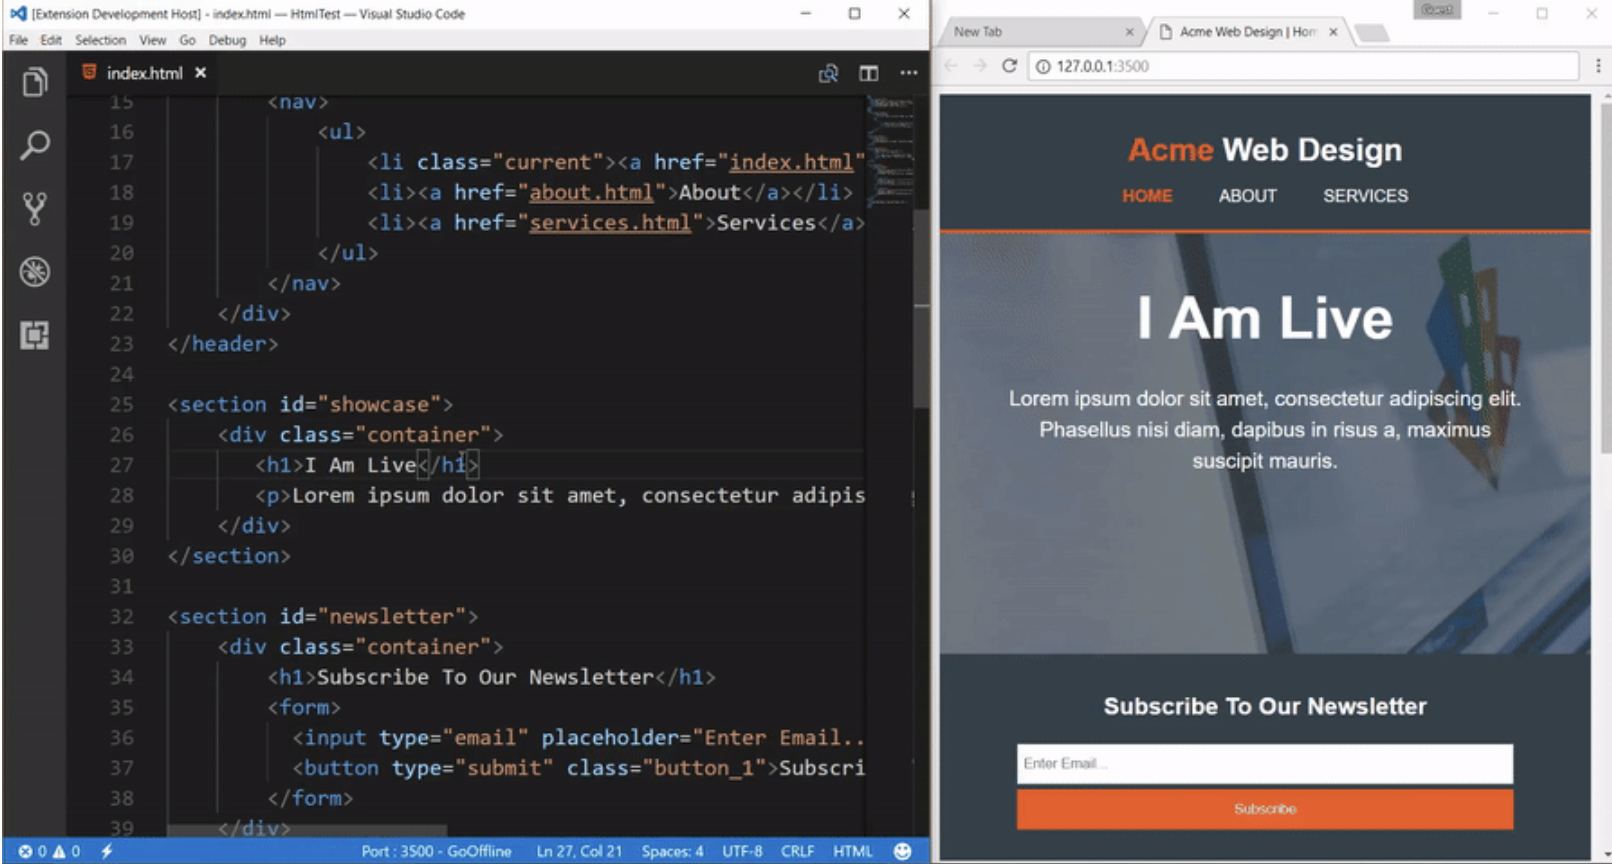
\includegraphics[width=10cm]{images/image04.png}
\end{center}

\subsection{Installation des dépendances}
Pour le moment, {\color{monOrange}create-vue} a déclaré toutes les dépendances et les configurations nécessaires en suivant vos options. Aucune dépendance {\tt JavaScript} n'a encore été installée par {\tt npm}. Pour les installer, il suffit d'ouvrir un terminal et d'aller dans le dossier de votre application, par exemple :
\begin{minted}[
mathescape,
framesep=2mm,
baselinestretch=1.2,
fontsize=\footnotesize,
bgcolor=LightGray,
%linenos
]{bash}
cd dymaproject
\end{minted}

Et ensuite de lancer l'installation des dépendances :
\begin{minted}[
mathescape,
framesep=2mm,
baselinestretch=1.2,
fontsize=\footnotesize,
bgcolor=LightGray,
%linenos
]{bash}
npm install
\end{minted}

\subsection{Utilisation du linter}
Un linter est un outil d'analyse de code qui permet de détecter les erreurs et les problèmes de syntaxe. La configuration du linter, en l'occurrence {\tt ESLint} est dans le fichier {\tt .eslintrc.cjs} :
\begin{minted}[
mathescape,
framesep=2mm,
baselinestretch=1.2,
fontsize=\footnotesize,
bgcolor=LightGray,
%linenos
]{javascript}
/* eslint-env node */
require('@rushstack/eslint-patch/modern-module-resolution')

module.exports = {
  root: true,
  'extends': [
    'plugin:vue/vue3-essential',
    'eslint:recommended',
    '@vue/eslint-config-typescript',
    '@vue/eslint-config-prettier/skip-formatting'
  ],
  parserOptions: {
    ecmaVersion: 'latest'
  }
}
\end{minted}

{\color{monOrange} create-vue} a donc automatiquement créé la bonne configuration du linter pour une utilisation avec {\tt Vue.js}. Pour exécuter le linter avec la configuration faites :

\begin{minted}[
mathescape,
framesep=2mm,
baselinestretch=1.2,
fontsize=\footnotesize,
bgcolor=LightGray,
%linenos
]{bash}
npm run lint
\end{minted}     

Cela exécutera le script {\tt lint} déclaré dans le fichier {\tt package.json}. Pour l'instant il y a bien sûr aucune indication car nous n'avons pas commencé à coder ! Mais exécuter cette commande de temps en temps lors du développement permet d'éviter certaines erreurs et de suivre les recommandations pour les bonnes pratiques en matière de syntaxe (appelées coding style).

\subsection{Lancer le serveur de développement}
Pour lancer le serveur de développement il suffit d'exécuter le script dev :
\begin{minted}[
mathescape,
framesep=2mm,
baselinestretch=1.2,
fontsize=\footnotesize,
bgcolor=LightGray,
%linenos
]{bash}
npm run dev
\end{minted} 

Cela va en fait exécuter {\color{monOrange}vite} qui va lancer son serveur de développement. Vous pourrez ainsi accéder à l'application {\tt Vue.js} dans votre navigateur à l'adresse {\color{monOrange} http://localhost:5173/}.

\begin{center}
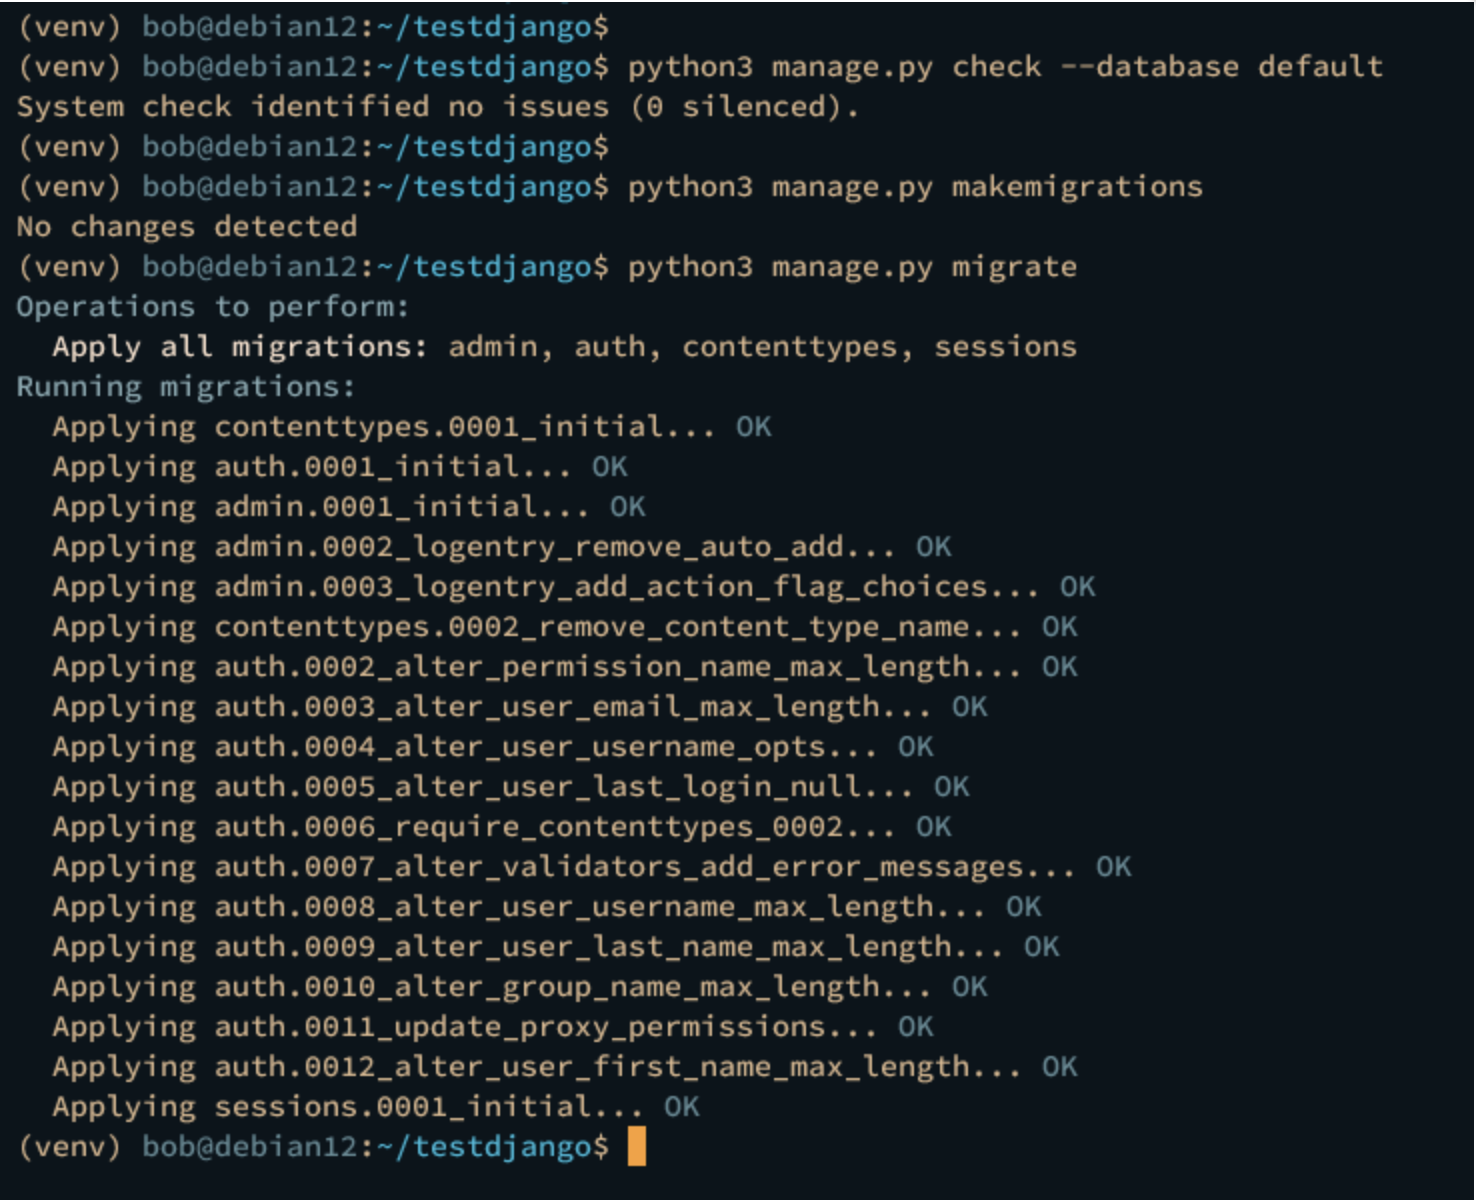
\includegraphics[width=10cm]{images/image13.png}
\end{center}

%%%%%%%%%%%%%%%%%%%%%%%%%%%%%%%%%%%%%%%%%%%%%%%%%%%%%%%%%%%%%%%%%
\section{Architecture initiale}
\subsection{Architecture initiale d'un projet généré par create-vue}
L'architecture initiale du projet généré est la suivante :
\begin{center}
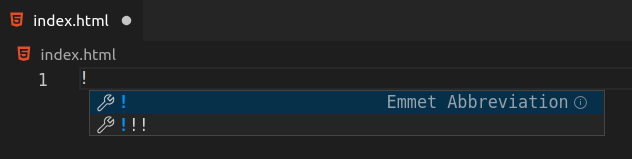
\includegraphics[width=3cm]{images/image05.png}
\end{center}

\subsection{Détail des fichiers et des dossiers}
\begin{itemize}
\item {\tt vite.config.js} : fichier de configuration de Vite.
\item {\tt tsconfig.node.json} : fichier de configuration de Vite pour pouvoir utiliser TypeScript. Vous pouvez retirer vitest, cypress, playwright de la propriété types car nous ne les utiliserons pas pour le moment :


\begin{minted}[
mathescape,
framesep=2mm,
baselinestretch=1.2,
fontsize=\footnotesize,
bgcolor=LightGray,
%linenos
]{javascript}
{
  "extends": "@vue/tsconfig/tsconfig.node.json",
  "include": ["vite.config.*"],
  "compilerOptions": {
    "composite": true,
    "types": ["node"]
  }
}
\end{minted} 
\item {\tt tsconfig.json} : fichier de configuration de TypeScript. Toutes les applications utilisant TypeScript ont ce fichier. Il permet de configurer notamment les options pour transpiler le TypeScript en JavaScript.
\item {\tt README.md} : décrit brièvement les différentes commandes possibles et la configuration recommandée de l'éditeur VS Code.
\item {\tt package.json} et {\tt package-lock.json} : ces fichiers {\tt JSON} permettent de décrire le projet et surtout de détailler les dépendances et leurs versions requises pour l'utiliser. Il décrit également les scripts pouvant être lancés avec {\color{monOrange}npm run}.
\end{itemize}
Les scripts disponibles sont :
\begin{itemize}
\item {\color{blue} dev} : qui permet de lancer le serveur de développement de {\color{monOrange} Vite} en local.
\item  {\color{blue} build} : qui permet de construire la version de l'application optimisée pour la production.
\item  {\color{blue} preview}  : qui permet de visualiser la version de production en local (par exemple avant de la mettre réellement en production sur des serveurs).
\item  {\color{blue} typecheck}  : qui permet de vérifier les types du code {\color{monOrange} TypeScript} sans transpiler le {\color{monOrange} TypeScript} en {\tt JavaScript}.
\item  {\color{blue} lint}  : qui permet d'exécuter {\color{monOrange} ESLint} avec les bonnes options.
\item  {\color{blue} index.html } : template {\tt HTML} qui sera envoyé au navigateur.
\item  {\color{blue} env.d.ts}  : fichier qui permet de charger des types supplémentaires pour utiliser {\color{monOrange} TypeScript} avec {\color{monOrange} Vue.js}.
\item  {\color{blue} .gitignore}  : permet de lister les fichiers qui ne doivent pas être pris en compte par {\color{monOrange} Git}.

\item  {\color{blue} .eslintrc}  : fichier de configuration de {\color{monOrange} ESLint} que nous avons déjà expliqué.
\item  {\color{blue} src } : dossier qui contient les fichiers sources de votre application (d'où le nom {\color{monOrange} src} pour source).
\item  {\color{blue} public}  : dossier qui contient les fichiers qui n'ont pas besoin d'être traité par {\color{monOrange} Vite} ou par aucun outil et qui sont directement envoyés par le serveur au navigateur.
\item  {\color{blue} src/main.ts}  : il s'agit du point d'entrée de notre application. Nous expliquerons plus loin dans le cours la fonction {\tt createApp()} ainsi que {\tt \$mount}. Sachez simplement que nous importons notre composant racine {\color{monOrange} App} et créons l'instance racine de l'application ici.
\item  {\color{blue} src/App.vue}  : il s'agit du composant référencé dans {\color{monOrange} main.ts} qui constitue la racine des vues de notre application. Il s'agit du premier composant rendu, et de lui découle les rendus de tous les autres composants. Nous étudierons la structure des composants dans une prochaine leçon.
\item  {\color{blue} src/components}  : dossier qui contient les composants de notre application {\color{monOrange} Vue}.
\item  {\color{blue} src/components/HelloWorld.vue}  : sous-composant de {\color{monOrange} App.vue}.
\item  {\color{blue} src/assets}  : dossier contenant les ressources de l'application comme les images, le {\tt CSS} etc.
\item  {\color{blue} node\_modules}  : contient toutes les dépendances installées par {\color{monOrange} npm}.
\end{itemize}

%%%%%%%%%%%%%%%%%%%%%%%%%%%%%%%%%%%%%%%%%%%%%%%%%%%%%%%%%%%%%%%%%%%%%%%%%


\section{Comment fonctionne Vue ?}
Nous allons voir les fichiers par ordre logique. Le navigateur reçoit en premier l'{\color{monOrange}index.html}.

\subsection{Le fichier {\color{monOrange}index.html}}
Le fichier index.html est ce que le navigateur va lire en premier :
\begin{minted}[
mathescape,
framesep=2mm,
baselinestretch=1.2,
fontsize=\footnotesize,
bgcolor=LightGray,
%linenos
]{html}
<!DOCTYPE html>
<html lang="en">
  <head>
    <meta charset="UTF-8" />
    <link rel="icon" href="/favicon.ico" />
    <meta name="viewport" content="width=device-width, initial-scale=1.0" />
    <title>Vite App</title>
  </head>
  <body>
    <div id="app"></div>
    <script type="module" src="/src/main.ts"></script>
  </body>
</html>
\end{minted} 

Notez bien qu'il y a une {\tt div} conteneur avec l'{\color{monOrange}id app}. Notez également que le fichier src/main.ts est chargé comme un module {\tt JavaScript}. Le navigateur demande donc ce module au serveur.

\subsection{Le fichier {\color{monOrange}src/main.ts}}
Le fichier {\color{monOrange}main.ts} est le point d'entrée de l'application car c'est le premier fichier {\tt JavaScript} chargé par le navigateur.

Note : le fichier est en {\color{monOrange}.ts} car c'est un fichier {\tt TypeScript} mais il sera transpilé par Vite en {\tt JavaScript} que ce soit pour le développement ou la production. En effet, le navigateur ne comprend que le langage {\tt JavaScript} et pas le {\tt TypeScript}.
\begin{minted}[
mathescape,
framesep=2mm,
baselinestretch=1.2,
fontsize=\footnotesize,
bgcolor=LightGray,
%linenos
]{javascript}
import { createApp } from "vue";
import App from "./App.vue";

createApp(App).mount("#app");
\end{minted} 

{\tt import App from "./App.vue";} permet d'importer le composant {\color{monOrange}App} que nous verrons juste après. {\tt createApp()} permet de créer une instance de votre application {\color{monOrange}Vue.js}. Elle prend en argument, le composant racine, c'est-à-dire le premier composant de votre application qui aura d'autres composants enfants.

{\tt mount()} permet de monter l'application instanciée par {\tt createApp()} dans un conteneur qui est identifié par un sélecteur {\tt CSS}. Ici, cela signifie que le composant racine {\color{monOrange}App} sera monté sur le conteneur dont l'{\color{monOrange}id} est {\color{monOrange}app} :
\begin{minted}[
mathescape,
framesep=2mm,
baselinestretch=1.2,
fontsize=\footnotesize,
bgcolor=LightGray,
%linenos
]{html}
<div id="app"></div>
\end{minted} 

Le composant sera ainsi affiché (on dit plus souvent rendu) dans ce conteneur.

\subsection{Le fichier {\color{monOrange}src/App.vue}}
Le fichier {\tt App.vue} est le composant racine. C'est le premier composant de l'application qui est chargé et instancié par {\tt createApp()}. Ce composant est le sommet de ce qu'on appelle l'arbre des composants : à savoir l'organisation hiérarchique des composants de l'application. Une application a des dizaines voir des centaines de composants qui sont organisés en arbre à partir du composant racine :
\begin{center}
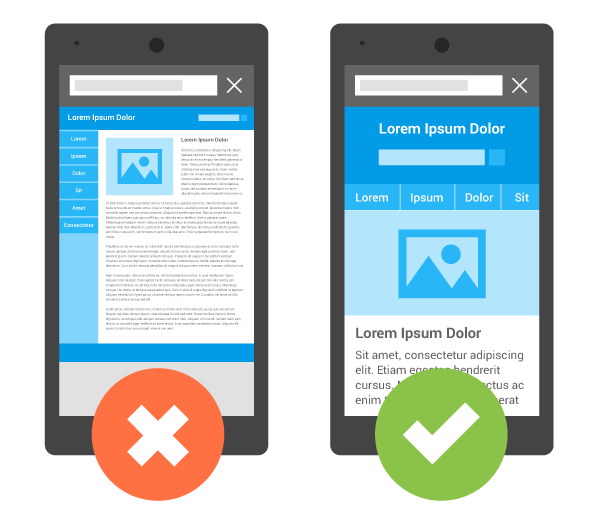
\includegraphics[width=12cm]{images/image06.png}
\end{center}

Remarquez déjà que le composant {\color{monOrange}App.vue} est constitué de trois parties : {\tt template, script} et {\tt style}. Nous étudierons bientôt les composants en détail.

\subsection{Aller plus loin sur le fonctionnement de Vue.js : le {\color{monOrange}DOM virtuel}}
Nous allons d'abord effectuer quelques rappels avant d'approfondir le fonctionnement de Vue.js.
\subsubsection{Le DOM (Document Object Model)}
Le {\tt DOM} permet de passer du {\tt HTML} à un grand objet document qui est un arbre regroupant tous les éléments déclarés en {\tt HTML}. Autrement dit, lorsque le navigateur reçoit le {\tt HTML} de la page, il va le parser (c'est-à-dire l'analyser) et le transformer en {\tt DOM} grâce à des algorithmes. Ainsi, les attributs {\tt HTML} deviennent automatiquement des propriétés des objets du {\tt DOM}. Par exemple :
\begin{minted}[
mathescape,
framesep=2mm,
baselinestretch=1.2,
fontsize=\footnotesize,
bgcolor=LightGray,
%linenos
]{html}
<body id="page">
\end{minted} 

Devient un nœud sur l'objet document qui sera un objet body contenant une propriété id contenant la valeur page.

Il existe plusieurs types de noeuds :
\begin{center}
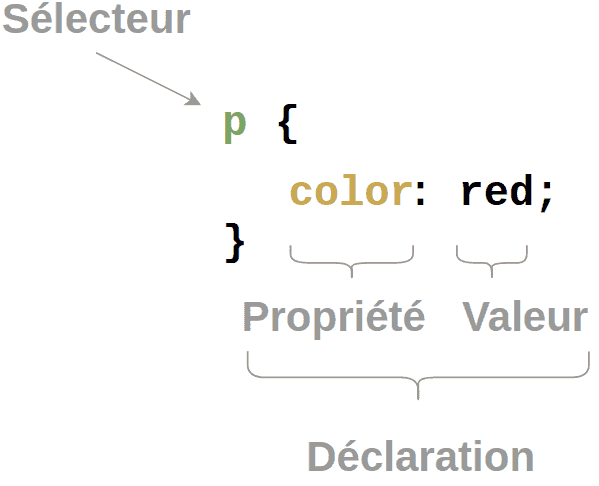
\includegraphics[width=15cm]{images/image07.png}
\end{center}

\subsubsection{Le DOM virtuel}
Dans les applications Web modernes, il peut y avoir des centaines ou des milliers de nœuds sur lesquels sont enregistrés de nombreux gestionnaires d'événements. En conséquence, de très nombreuses mises à jour du {\tt DOM} doivent être réalisées. Or, ces mises à jour sont très coûteuses en performance car plus le {\tt DOM} est grand, plus les recherches et les changements sont coûteux. {\color{monOrange}Vue.js} utilise donc un {\tt DOM} virtuel (appelé {\tt VDOM}) qui est une représentation du {\tt DOM} en {\tt JavaScript}. Le {\tt DOM } virtuel n'est donc qu'un simple, immense, objet {\tt JavaScript} :
\begin{minted}[
mathescape,
framesep=2mm,
baselinestretch=1.2,
fontsize=\footnotesize,
bgcolor=LightGray,
%linenos
]{javascript}
const vnode = {
  type: 'div',
  props: {
    id: 'hello'
  },
  children: [
    /* plein de vnodes */
  ]
}
\end{minted} 

Les noeuds du DOM virtuels sont appelés des noeuds virtuels ou {\color{monOrange}vnode} (pour virtual node). {\color{monOrange}Vue.js} va transformer le {\tt VDOM} en {\tt DOM} pour que le navigateur puisse afficher la page. Ce processus est appelé le montage (mount en anglais).

Lorsque des mises à jour sur la page doivent intervenir, le {\tt DOM} virtuel est modifié avant que les modifications sur le {\tt DOM} ne soient effectuées. Le {\tt DOM} virtuel est une représentation légère du {\tt DOM} en {\tt JavaScript} qui peut être utilisée par des algorithmes très performants de comparaison des différences entre {\tt DOM} virtuel et {\tt DOM}.

Dès lors que le {\tt DOM} doit être modifié, un patch est appliqué par {\color{monOrange}Vue.js} de manière extrêmement optimisée pour ne réaliser que les changements absolument nécessaires. Par exemple, si aucune valeur affichée ne change, alors aucune mise à jour du {\tt DOM} n'est déclenchée ce qui économise beaucoup en performance.

En résumé, {\color{monOrange}Vue.js} va créer au départ un {\tt DOM} virtuel puis le convertir en {\tt DOM HTML} pour l'affichage lors du montage. Lorsque des changements interviennent, par exemple un événement survient, les changements affectant le {\tt DOM} virtuel sont analysés par des algorithmes et seuls les changements ayant un effet sur l'affichage sont propagés au {\tt DOM} lors de la phase de mise à jour (patch ou diffing en anglais). Ainsi, seules les insertions, les modifications et les suppressions d'éléments {\tt HTML} absolument nécessaires sont effectuées, ce qui permet un énorme gain de performance.

%%%%%%%%%%%%%%%%%%%%%%%%%%%%%%%%%%%%%%%%%%%%%%%%%%%%%%%%%%%

\section{Les API composition et options}
{\color{monOrange}Vue.js} propose deux API pour écrire des composants {\color{monOrange}Vue} : l'API options et l'API composition.
\begin{itemize}
\item L'API options est l'API originelle qui existe depuis la première version du {\color{monOrange}framework}.
\item L'API composition est l'API avec laquelle {\color{monOrange}Vue} a été réécrite pour la version 3. C'est la nouvelle API qui est aujourd'hui recommandée et celle que nous verrons dans la formation.
\end{itemize}
\subsection{L'API options}
Dans l'ancienne API options, la logique du composant est définie dans un objet comportant des options comme {\tt data}, {\tt methods} ou {\tt mounted} par exemple. Les propriétés sont définies sur l'objet {\tt this} disponible dans les options.

Nous ne détaillerons pas plus car ce n'est pas l'API que nous utiliserons. Nous la présentons uniquement pour que vous puissiez la reconnaître lorsque vous la rencontrez. Voici à quoi ressemble un composant écrit avec l'API options :
\begin{minted}[
mathescape,
framesep=2mm,
baselinestretch=1.2,
fontsize=\footnotesize,
bgcolor=LightGray,
%linenos
]{html}
<script>
export default {
  data() {
    return {
      count: 0
    }
  },
  methods: {
    increment() {
      this.count++
    }
  },
  mounted() {
    console.log(`La valeur initiale est ${this.count}.`)
  }
}
</script>

<template>
  <button @click="increment">Valeur du compteur : {{ count }}</button>
</template>
\end{minted} 

\subsection{L'API composition}
Avec l'API composition nous définissons la logique d'un composant en important des fonctions. Voilà le même exemple avec la nouvelle API :
\begin{minted}[
mathescape,
framesep=2mm,
baselinestretch=1.2,
fontsize=\footnotesize,
bgcolor=LightGray,
%linenos
]{html}
<script setup>
import { ref, onMounted } from 'vue'

const count = ref(0)
function increment() {
  count.value++
}

onMounted(() => {
  console.log(`La valeur initiale est ${count.value}.`)
})
</script>

<template>
  <button @click="increment">Valeur du compteur : {{ count }}</button>
</template>
\end{minted} 

\subsection{Les {\color{monOrange}Single-File Components} (SFC)}
Les SFC sont des composants écrits dans des fichiers qui terminent par l'extension {\color{monOrange}.vue}. Un SFC comporte la logique du composant (partie script en {\tt JavaScript/TypeScript}), le template (en {\tt HTML}) et le style (en {\tt CSS} ou {\tt Sass}).

Il est fortement recommandé d'utiliser les SFC pour écrire des composants {\color{monOrange}Vue.js}. C'est d'ailleurs ce que nous utiliserons tout le long de la formation.

%%%%%%%%%%%%%%%%%%%%%%%%%%%%%%%%%%%%%%%%%%%%%%%%%%%%%%%

\section{Création d'un composant}
\subsection{Passer en mode {\color{monOrange}Take Over}}
L'extension {\color{monOrange}Volar} est plus performante pour gérer l'utilisation de {\tt TypeScript} avec {\color{monOrange}Vue.js}. Aussi, il faut configurer l'éditeur {\tt VS Code} pour lui dire que nous utilisons {\color{monOrange}Volar}.

Pour ce faire, aller sur l'onglet {\tt Extensions de VS Code}. Recherchez {\tt @builtin typescript}. Cliquez sur {\tt TypeScript and JavaScript Language Features}. Cliquez sur {\tt Désactiver (espace de travail)}. Cela désactivera uniquement pour ce projet. Cliquez ensuite sur Rechargement requis.

\subsection{Utilisation du mode {\color{monOrange}strict} de {\color{monOrange}TypeScript}}
Pour activer l'option {\color{monOrange}strict} du compilateur {\tt TypeScript} modifiez le fichier {\tt tsconfig.json} :
\begin{minted}[
mathescape,
framesep=2mm,
baselinestretch=1.2,
fontsize=\footnotesize,
bgcolor=LightGray,
%linenos
]{javascript}
{
  "extends": "@vue/tsconfig/tsconfig.web.json",
  "include": ["env.d.ts", "src/**/*", "src/**/*.vue"],
  "compilerOptions": {
    "strict": true,
    "baseUrl": ".",
    "paths": {
      "@/*": ["./src/*"]
    }
  },
  "references": [
    {
      "path": "./tsconfig.node.json"
    }
  ]
}
\end{minted} 

Cette option permet d'activer de nombreuses configurations plus strictes pour le contrôle des types par le compilateur. Cela permet d'améliorer sa capacité à détecter des erreurs.

\subsection{Création du premier composant}
Commençons par supprimer les composants mis en place automatiquement par {\color{monOrange}create-vue} pour la page de présentation lors du lancement de l'application. 
\begin{enumerate}
\item Supprimez tous les fichiers et les dossiers dans {\tt src/components/}.
\item Supprimez le contenu, mais pas le fichier de {\tt src/App.vue}.
\end{enumerate}

Comme nous l'avons vu, un composant {\color{blue} monofichier} (SFC, pour Single-file component) est un fichier {\color{blue} .vue} dont le nom est par convention en {\tt PascalCase}. Un composant monofichier a donc un template qui comporte le {\tt HTML}, une partie script qui comporte le JavaScript et une partie style qui comporte le {\tt CSS}. Voici l'exemple minimal de la vidéo :
\begin{minted}[
mathescape,
framesep=2mm,
baselinestretch=1.2,
fontsize=\footnotesize,
bgcolor=LightGray,
%linenos
]{html}
<template>
    <h1>Bonjour {{name}}</h1>
</template>

<script setup lang="ts">
    const name = 'Jean';
</script>

<style></style>
\end{minted} 

%\subsection{Exemple exécutable}
%Vous pouvez aussi directement utiliser ce code exécutable. N'hésitez pas à l'ouvrir dans un nouvel onglet :

%%%%%%%%%%%%%%%%%%%%%%%%%%%%%%%%%%%%%%%%%%%%%%%%%%%%%%

\section{Vue.js sans Vite}
\subsection{Utiliser {\color{monOrange}Vue.js} sans {\color{monOrange}Vite}}
Créez un dossier projet-vue.

Dans ce dossier, créez un fichier index.html :
\begin{minted}[
mathescape,
framesep=2mm,
baselinestretch=1.2,
fontsize=\footnotesize,
bgcolor=LightGray,
%linenos
]{html}
<!DOCTYPE html>
<html lang="en">
  <head>
    <meta charset="UTF-8" />
    <meta http-equiv="X-UA-Compatible" content="IE=edge" />
    <meta name="viewport" content="width=device-width, initial-scale=1.0" />
    <title>Document</title>
    <script src="https://unpkg.com/vue@3"></script>
  </head>
  <body>
    <div id="app">
      <h1>Bonjour {{ name }}</h1>
    </div>

    <script>
      Vue.createApp({
        setup() {
          const name = 'test';
          return {
            name,
          };
        },
      }).mount('#app');
    </script>
  </body>
</html>
\end{minted} 

Ici, nous n'utilisons que la librairie {\color{monOrange}Vue.js} sans {\color{monOrange}Vite} et sans aucune autre librairie. 
\begin{itemize}
\item Il n'y a aucune étape de {\tt build}, nous ne pouvons pas utiliser Sass, TypeScript etc.

\item Il n'y a pas de minification du code et pleins d'avantages apportés par {\color{monOrange}Vite}.
\end{itemize}
Cet exemple permet simplement de montrer comment utiliser {\color{monOrange}Vue.js} seul mais dans toute la formation nous n'utiliserons pas du tout cette méthode car il est impossible d'écrire une application complexe comme cela. Cette manière de faire peut être utile pour par exemple gérer une barre de recherche sur une application avec {\color{monOrange}Symfony} côté serveur.

	\chapter{Intéragir avec le DOM}
	\section{Introduction aux directives}
\subsection{Les directives}
Les directives sont des attributs spéciaux avec le préfixe {\color{monOrange}v-}. L'objectif d'une directive est d'appliquer de manière réactive des effets au {\tt DOM} lorsque la valeur de son expression change. Les directives natives sont les suivantes :
\begin{itemize}
\item v-text (qui équivaut à {{ }})
\item v-bind
\item v-html
\item v-once
\item v-show
\item v-if
\item v-else
\item v-else-if
\item v-for
\item v-on
\item v-model
\item v-pre
\item v-cloak
\item v-slot
\item v-memo
\end{itemize}

Il est également possible, comme nous l'étudierons, de créer ses propres directives {\color{monOrange}Vue}. Commençons par la directive la plus simple v-text.

\subsection{La directive {\color{monOrange}v-text} et l'interpolation de texte}
La directive {\color{monOrange}v-text} permet de mettre à jour le contenu de la propriété textContent de l'élément {\tt HTML}. La directive prend en argument la propriété déclarée sur le composant dont la valeur doit être utilisée. On appelle cela l'interpolation de texte. Par exemple, s'il existe une propriété message sur le composant dans la partie script, alors nous pouvons utiliser la directive de cette manière côté template :
\begin{minted}[
mathescape,
framesep=2mm,
baselinestretch=1.2,
fontsize=\footnotesize,
bgcolor=LightGray,
%linenos
]{html}
<span v-text="message"></span>
\end{minted}

La propriété {\color{blue}textContent} de l'élément {\tt span} sera alors remplacé par la valeur de la propriété {\tt message}. Comme lier une propriété est extrêmement courant, il existe une forme raccourcie appelée la notation moustache (de part sa forme), utilisant deux paires d'accolades :
\begin{minted}[
mathescape,
framesep=2mm,
baselinestretch=1.2,
fontsize=\footnotesize,
bgcolor=LightGray,
%linenos
]{html}
<span>{{message}}</span>
\end{minted}

Est du sucre syntaxique pour :
\begin{minted}[
mathescape,
framesep=2mm,
baselinestretch=1.2,
fontsize=\footnotesize,
bgcolor=LightGray,
%linenos
]{html}
<span v-text="message"></span>
\end{minted}

Note : en programmation, on appelle sucre syntaxique une syntaxe plus concise ou plus élégante qui est remplacée automatiquement par le code complet et donne le même résultat qu'une expression plus longue.

\subsection{Utilisation d'expression JavaScript}
Avec {\color{monOrange}Vue.js} il est possible d'utiliser toute expression {\tt JavaScript} valide comme argument d'une directive. Voici un exemple avec un ternaire :
\begin{minted}[
mathescape,
framesep=2mm,
baselinestretch=1.2,
fontsize=\footnotesize,
bgcolor=LightGray,
%linenos
]{javascript}
{{ condition ? 'Oui' : 'Non' }}
\end{minted}
Autre exemple :
\begin{minted}[
mathescape,
framesep=2mm,
baselinestretch=1.2,
fontsize=\footnotesize,
bgcolor=LightGray,
%linenos
]{javascript}
{{ message.reverse().toUpperCase() }}
\end{minted}

Encore un autre :
\begin{minted}[
mathescape,
framesep=2mm,
baselinestretch=1.2,
fontsize=\footnotesize,
bgcolor=LightGray,
%linenos
]{html}
<h1>Bonjour {{ `${prenom.toLowerCase()} ${nom.toUpperCase()}`}}</h1>
\end{minted}

Nous verrons énormément d'exemples au cours de la formation.

%Exemple exécutable
%Vous pouvez aussi directement utiliser ce code exécutable. N'hésitez pas à l'ouvrir dans un nouvel onglet :

\section{Directive {\color{monOrange}v-html}}
La directive {\color{monOrange}v-html} permet de mettre à jour l'attribut {\color{monOrange}innerHTML} d'un élément. Le contenu sera inséré comme du HTML simple.

Attention ! Le rendu dynamique de HTML sur votre site Web peut être très dangereux car il peut facilement conduire à des attaques {\tt XSS}. Utilisez uniquement {\color{monOrange}v-html} sur un contenu sûr et jamais sur du contenu fourni par l'utilisateur. Voici un exemple :
\begin{minted}[
mathescape,
framesep=2mm,
baselinestretch=1.2,
%fontsize=\footnotesize,
bgcolor=LightGray,
%linenos
]{html}
<p>Contenu HTML: <span v-html="varHtml"></span></p>
\end{minted}

%Exemple exécutable
%Vous pouvez aussi directement utiliser ce code exécutable. N'hésitez pas à l'ouvrir dans un nouvel onglet :

\section{Liaison de propriété avec v-bind}
La directive v-bind permet d'associer dynamiquement un attribut à une propriété.
\subsection{Syntaxe de base}
Elle prend en argument l'attribut auquel la propriété est liée. Ainsi par exemple :
\begin{minted}[
mathescape,
framesep=2mm,
baselinestretch=1.2,
%fontsize=\footnotesize,
bgcolor=LightGray,
%linenos
]{html}
<a v-bind:href="url"></a>
\end{minted}

L'attribut href de l'ancre est liée ici à la valeur de la variable url grâce à l'utilisation de la directive v-bind.

\subsection{Syntaxe raccourcie}
Comme cette directive est extrêmement utilisée, il existe une forme raccourcie :
\begin{minted}[
mathescape,
framesep=2mm,
baselinestretch=1.2,
%fontsize=\footnotesize,
bgcolor=LightGray,
%linenos
]{html}
<a :href="url"></a>
\end{minted}
C'est cette forme que nous utiliserons dans la formation et qui est recommandée.
\subsection{Utilisation sur des attributs booléens}
Les attributs booléens sont les attributs pour lesquels la simple présence de l'attribut représente la valeur true et leur absence la valeur false. Il y en a 26 différents.

Des exemples sont : disabled, checked, multiple, readonly, selected, hidden etc. Lorsque la directive v-bind est utilisée sur un attribut booléen, le comportement est le suivant : si la variable liée vaut true alors l'attribut sera ajouté par Vue.js automatiquement, si la variable vaut false alors l'attribut sera retiré. Par exemple :

\begin{minted}[
mathescape,
framesep=2mm,
baselinestretch=1.2,
%fontsize=\footnotesize,
bgcolor=LightGray,
%linenos
]{html}
<button :disabled="isButtonDisabled">Button</button>
\end{minted}

Si isButtonDisabled vaut true alors l'attribut disabled sera ajouté par Vue.js sur le DOM, s'il vaut false il sera enlevé.

\subsection{Utilisation sur plusieurs attributs}
La directive v-bind peut être utilisée pour lier un objet contenant des paires nom-valeur d'attribut. Exemple :
\begin{minted}[
mathescape,
framesep=2mm,
baselinestretch=1.2,
%fontsize=\footnotesize,
bgcolor=LightGray,
%linenos
]{html}
<div v-bind="{ id: propriété, 'autre-attribut': autrePropriété }"></div>
\end{minted}

Ainsi, si nous avons côté script :
\begin{minted}[
mathescape,
framesep=2mm,
baselinestretch=1.2,
%fontsize=\footnotesize,
bgcolor=LightGray,
%linenos
]{javascript}
const objet = {
  id: 'container',
  class: 'container'
}
\end{minted}

Nous pouvons lier cet objet avec la directive v-bind :
\begin{minted}[
mathescape,
framesep=2mm,
baselinestretch=1.2,
%fontsize=\footnotesize,
bgcolor=LightGray,
%linenos
]{html}
<div v-bind="objet"></div>
\end{minted}

Attention ! Dans ce cas la notation raccourcie n'est pas possible.
\subsection{Utilisation avec class et style}
Lorsqu'elle est utilisée avec les attributs class ou style, la directive v-bind peut prendre un tableau ou un objet en argument de cette façon :
\begin{minted}[
mathescape,
framesep=2mm,
baselinestretch=1.2,
%fontsize=\footnotesize,
bgcolor=LightGray,
%linenos
]{html}
<div :style="{ fontSize: size + 'px' }"></div>
\end{minted}
Ou :
\begin{minted}[
mathescape,
framesep=2mm,
baselinestretch=1.2,
%fontsize=\footnotesize,
bgcolor=LightGray,
%linenos
]{html}
<div :class="[classA, classB]"></div>
\end{minted}

Nous verrons des exemples dans la formation.

\subsection{Utilisation avec un attribut dynamique}
Vous pouvez utiliser une liaison dynamique également sur l'attribut avec cette syntaxe :
\begin{minted}[
mathescape,
framesep=2mm,
baselinestretch=1.2,
%fontsize=\footnotesize,
bgcolor=LightGray,
%linenos
]{html}
<button :[clé]="valeur"></button>
\end{minted}
Ici l'attribut peut être modifié dynamiquement en modifiant la valeur de la variable clé.

%Exemple exécutable
%Vous pouvez aussi directement utiliser ce code exécutable. N'hésitez pas à l'ouvrir dans un nouvel onglet :

\section{Utilisation de fonction dans les liaisons}
Comme nous l'avons vu, il est possible d'utiliser des expressions {\tt JavaScript} dans les templates. Nous pouvons donc invoquer des fonctions. Il est donc courant de voir :
\begin{minted}[
mathescape,
framesep=2mm,
baselinestretch=1.2,
%fontsize=\footnotesize,
bgcolor=LightGray,
%linenos
]{html}
<span :title="toTitleCase(titre)">
  {{ formatDate(date) }}
</span>
\end{minted}

Ici, nous utilisons deux invocations de fonction. L'une avec {\color{monOrange}v-bind} et l'autre avec {\color{monOrange}v-text}. Nous verrons de nombreux exemples au cours de la formation car c'est très courant.

%Exemple exécutable
%Vous pouvez aussi directement utiliser ce code exécutable. N'hésitez pas à l'ouvrir dans un nouvel onglet :

\section{Notions de base TypeScript}
\subsection{Les types statiques}
{\color{monOrange}TypeScript} permet de tout taper statiquement : vos variables, vos fonctions (arguments, valeur de retour) et vos classes. Le langage ne vous force pas à taper, ce qui vous laisse totalement libre de le faire ou non et ainsi d'adopter progressivement le typage statique en fonction de votre apprentissage.

\subsection{L'inférence de types}
{\color{monOrange}TypeScript}  va détecter automatiquement le type de votre variable en regardant la valeur qui lui est assignée. Nous reviendrons en détails sur cette fonctionnalité très pratique, mais elle permet sans aucune ligne supplémentaire d'avoir ce résultat :
\begin{minted}[
mathescape,
framesep=2mm,
baselinestretch=1.2,
%fontsize=\footnotesize,
bgcolor=LightGray,
%linenos
]{javascript}
const obj = { width: 1, height: 2 };
const aire = obj.width * obj.heigth;
// Property 'heigth' does not exist on type '{ width: number; height: number; }'. Did you mean // 'height'?
\end{minted}

Ici {\color{monOrange}TypeScript}  a détecté qu'aucune propriété {\tt heigth} n'existait sur objet vous invite à vérifier que vous n'avez pas fait une erreur. Magique, non ?

\subsection{Les types}
Comme son nom l'indique et comme nous l'avons vu {\color{monOrange}TypeScript}  est avant tout un langage pour taper. Il est possible de taper absolument tout comme nous le verrons : que ce soit les variables mais aussi les retours de fonction ou des situations encore plus complexes.

Typer au début peut sembler fastidieux : il faut ajouter un peu de code à chaque fois. Mais les bénéfices se remarquent très vite et dans cet ordre souvent :
\begin{enumerate}
\item  Vous aurez moins de bugs lors de l'exécution car beaucoup auront été signalés lors de la compilation : typo dans les noms, erreurs dans les conditions, dans les arguments passés, dans les retours de fonction etc.

\item   {\color{blue} VS} Code vous fournira avec un survol de la souris plein d'informations sur vos fonctions : quels arguments sont attendus etc, et vous gagnerez un temps fou grâce à l'autocomplétion (car  {\color{monOrange}TypeScript}  aura toutes les propriétés sur vos objets etc).

\item   Lorsque vous serez sur un projet à plusieurs, vous pourrez lire et comprendre beaucoup plus vite le code des autres développeurs car vous verrez facilement ce que prend et ce que retourne chaque fonction, quels sont les types acceptés par chaque variable etc.

\end{enumerate}
Une fois les premiers jours, où cela semblera être une surcouche embêtante, passée, vous ne pourrez plus faire sans !

\subsection{Les types primitifs}
Nous allons commencer par les types les plus basiques : les primitifs !

Pour préciser un type en  {\color{monOrange}TypeScript}  nous utilisons la plupart du temps (nous verrons en détails les autres cas) cette syntaxe :
\begin{minted}[
mathescape,
framesep=2mm,
baselinestretch=1.2,
%fontsize=\footnotesize,
bgcolor=LightGray,
%linenos
]{javascript}
variable: type;
\end{minted}

Il est possible de simplement taper une variable sans rien assigner ou de taper et assigner directement :
\begin{minted}[
mathescape,
framesep=2mm,
baselinestretch=1.2,
%fontsize=\footnotesize,
bgcolor=LightGray,
%linenos
]{javascript}
variable: type;
variable: type = x;
\end{minted}

\subsubsection{Les chaînes de caractères :string}
Les chaînes de caractères en {\color{monOrange}TypeScript}  comprennent exactement comme en {\tt JavaScript} les guillemets simples ou doubles et les accents graves ( {\tt backticks}) :
\begin{minted}[
mathescape,
framesep=2mm,
baselinestretch=1.2,
%fontsize=\footnotesize,
bgcolor=LightGray,
%linenos
]{javascript}
let prenom: string = "Jean";
prenom = 'Paul';
prenom = `Patrick`;
\end{minted}

\subsubsection{Les nombres :number}
Tous les nombres valides en {\tt JavaScript} le sont en {\color{monOrange}TypeScript} :
\begin{minted}[
mathescape,
framesep=2mm,
baselinestretch=1.2,
%fontsize=\footnotesize,
bgcolor=LightGray,
%linenos
]{javascript}
let decimal: number = 42;
let flottant: number = 42.22;
let hexadecimal: number = 0x2A;
let binaire: number = 0b101010;
let octal: number = 0o52;
\end{minted}

\subsubsection{Les booléens :boolean}
Le type {\tt boolean} n'accepte que {\tt true} ou {\tt false}:
\begin{minted}[
mathescape,
framesep=2mm,
baselinestretch=1.2,
%fontsize=\footnotesize,
bgcolor=LightGray,
%linenos
]{javascript}
let actif: boolean;
actif = true;
actif = false;
\end{minted}

\subsection{Le type any}
Il est possible de ne pas connaître le type de variables. Ces valeurs peuvent provenir d'un contenu dynamique, par exemple de l'utilisateur ou d'une bibliothèque tierce.

Il est également possible que vous souhaitiez taper plus tard votre fonction ou variable ou que vous soyez en train de convertir un fichier {\tt JavaScript} en {\color{monOrange}TypeScript} et que vous mettiez les types peu à peu.

Dans ces cas, nous souhaitons désactiver la vérification de type. Pour ce faire, nous les étiquetons avec le type {\color{blue}any}.
\begin{minted}[
mathescape,
framesep=2mm,
baselinestretch=1.2,
%fontsize=\footnotesize,
bgcolor=LightGray,
%linenos
]{javascript}
let pasSur: any = 4;
pasSur = 'en fait une string';
\end{minted}

Lorsque vous commencez en {\color{monOrange}TypeScript} vous aurez tendance à beaucoup trop utiliser {\color{blue} any}. A chaque fois que vous ne saurez pas trop le type vous mettrez {\color{blue} any}. Au début ce n'est pas très grave mais il faut vous forcer à faire l'effort de tout bien typer pour garder les bénéfices de l'usage de  {\color{monOrange}TypeScript}. Nous vous recommandons de ne quasiment jamais utiliser {\color{blue} any} sauf dans les cas vus ci-dessus.

\subsection{Le type {\color{monOrange}object}}
Le type {\color{monOrange}objet} permet simplement de représenter le type {\color{blue}non primitif} : tout ce qui n'est pas {\tt number, string, boolean, bigint, symbol, null} ou {\tt undefined}. Cela peut donc être un tableau, un objet littéral, etc.
\begin{minted}[
mathescape,
framesep=2mm,
baselinestretch=1.2,
%fontsize=\footnotesize,
bgcolor=LightGray,
%linenos
]{javascript}
let monObj: object;
monObj = {};
\end{minted}

Notez que {\color{monOrange}object} et {\color{monOrange}{}} sont deux manières de typer un objet, nous pouvons écrire :
\begin{minted}[
mathescape,
framesep=2mm,
baselinestretch=1.2,
%fontsize=\footnotesize,
bgcolor=LightGray,
%linenos
]{javascript}
let monObj: {};
monObj = {};
\end{minted}

\subsection{Le type {\color{monOrange}array}}
Il y a deux syntaxes en {\tt TypeScript} pour taper les {\color{monOrange}tableaux} . En {\tt TypeScript} un tableau est un tableau {\tt JavaScript} contenant un nombre indéfini d'éléments . Première possibilité :
\begin{minted}[
mathescape,
framesep=2mm,
baselinestretch=1.2,
%fontsize=\footnotesize,
bgcolor=LightGray,
%linenos
]{javascript}
type[];
\end{minted}

Où type est le type des éléments contenus dans un tableau. Il est possible d'accepter par exemple que les nombres :
\begin{minted}[
mathescape,
framesep=2mm,
baselinestretch=1.2,
%fontsize=\footnotesize,
bgcolor=LightGray,
%linenos
]{javascript}
let liste: number[] = [1, 2, 3];
\end{minted}
Tous les types :
\begin{minted}[
mathescape,
framesep=2mm,
baselinestretch=1.2,
%fontsize=\footnotesize,
bgcolor=LightGray,
%linenos
]{javascript}
let liste: any[] = [1, true, {}];
\end{minted}

\subsection{Qu'est-ce qu'une {\color{monOrange}interface} ?}
Une {\color{monOrange}interface} est un contrat qui définit la forme qui doit prendre un objet {\tt JavaScript} (objets littéraires, classes et fonctions) . Il est important de noter qu'une {\color{monOrange}interface} n'est pas compilée : aucun code {\tt JavaScript} ne sera créé à partir de l'interface. Elle sert uniquement pour l' IDE, c'est-à-dire pour {\color{blue}VS Code}, (auto-complétions et erreurs de types) et lors de la compilation.

\subsubsection{Notre première interface}
Prenons un premier exemple avec un objet :
\begin{minted}[
mathescape,
framesep=2mm,
baselinestretch=1.2,
%fontsize=\footnotesize,
bgcolor=LightGray,
%linenos
]{javascript}
interface User {
    prenom: string;
}
\end{minted}

Ici, notre objet {\color{monOrange}User} doit obligatoirement avoir une propriété {\color{blue}prenom} contenant une chaîne de caractères. Ensuite nous pouvons utiliser l' interface pour taper par exemple un paramètre d'une fonction :
\begin{minted}[
mathescape,
framesep=2mm,
baselinestretch=1.2,
%fontsize=\footnotesize,
bgcolor=LightGray,
%linenos
]{javascript}
function printUser(user: User) {
    console.log(user.prenom);
}
\end{minted}

Ici, la fonction {\color{blue}printUser} doit recevoir en argument un objet respectant l' interface {\color{monOrange}User} . Par exemple :
\begin{minted}[
mathescape,
framesep=2mm,
baselinestretch=1.2,
%fontsize=\footnotesize,
bgcolor=LightGray,
%linenos
]{javascript}
let paul = {prenom: 'Paul'};
printUser(paul);
\end{minted}

Attention ! Lorsque vous tapez le paramètre de cette manière {\tt user: User} , cela revient à dire que le paramètre doit au moins avoir le ou les propriétés de l'interface {\color{blue}User} et donc avoir une propriété {\tt prenom}.

En revanche, lorsque vous tapez un objet avec une interface, il faut que l'objet respecte exactement l'interface . C'est-à-dire qu'il doit avoir exactement les propriétés définies, ni plus ni moins. Voici un exemple pour bien comprendre :
\begin{minted}[
mathescape,
framesep=2mm,
baselinestretch=1.2,
%fontsize=\footnotesize,
bgcolor=LightGray,
%linenos
]{javascript}
interface User {
    prenom: string;
}

function printUser(user: User) {
    console.log(user.prenom);
}

const paul = {prenom: 'Paul', nom: 'Dupont'};

printUser(paul); // Cela fonctionne car paul a au moins une propriété nom

const jean: User = {prenom: 'Jean', nom: 'Duprey'}; // Erreur
\end{minted}

Dans le cas de l'objet {\color{blue} Jean}, {\tt TypeScript} nous signalons l'erreur suivante : {\bf Type '{ prenom: string; nom: string; }' is not assignable to type 'User'. Object literal may only specify known properties, and 'nom' does not exist in type 'User'}.

Autrement dit, il se plaint car {\color{blue} Jean} a une propriété {\tt nom} qui ne respecte pas le contrat imposé par l' interface {\color{monOrange} User}.

\subsubsection{Les propriétés optionnelles avec?}
Il est possible de définir des propriétés optionnelles comme nous l'avons vu pour les arguments de fonction en utilisant {\color{monOrange} ?}. Ces propriétés sont également utilisables dans les interfaces.
\begin{minted}[
mathescape,
framesep=2mm,
baselinestretch=1.2,
%fontsize=\footnotesize,
bgcolor=LightGray,
%linenos
]{javascript}
interface User {
  prenom: string;
  nom?: string;
}
\end{minted}

Ici, nous établissons comme contrat que les objets qui respecteront l' {\color{monOrange}interface User} auront obligatoirement une propriété {\tt prenom} contenant une chaîne de caractères, et une propriété optionnelle {\tt nom}, qui si elle existe, devra également contenir une chaîne de caractères. En outre, les propriétés optionnelles permettent l'autocomplétion et l'autocorrection.

\subsection{Les unions de type}
Les unions de type permettent de combiner deux ou plusieurs types et s'utilisent avec {\color{monOrange}|} . Les unions s'utilisent dans toutes les situations.

\subsubsection{Unions de type et variables}
Prenons un premier exemple :
\begin{minted}[
mathescape,
framesep=2mm,
baselinestretch=1.2,
%fontsize=\footnotesize,
bgcolor=LightGray,
%linenos
]{javascript}
let uneVar: string | number;}
\end{minted}

Ici, nous effectuons une union entre les types de chaîne de caractères et de nombres. La variable pourra ainsi recevoir l'un des deux types.

\subsubsection{Unions de type et fonctions}
Vous pouvez également taper les paramètres des fonctions en utilisant des unions :
\begin{minted}[
mathescape,
framesep=2mm,
baselinestretch=1.2,
%fontsize=\footnotesize,
bgcolor=LightGray,
%linenos
]{javascript}
function ajouter(a: string | number, b: string | number) {
  return Number(a) + Number(b);
}
\end{minted}

Ici par exemple, notre fonction peut ajouter des nombres et des chaînes de caractères. Nous voulons donc utiliser des unions pour les paramètres de la fonction. Vous pouvez également taper les retours de fonctions en utilisant des unions :
\begin{minted}[
mathescape,
framesep=2mm,
baselinestretch=1.2,
%fontsize=\footnotesize,
bgcolor=LightGray,
%linenos
]{javascript}
function ajouter(isAdmin: boolean): string | void {
  if (isAdmin) {
    return 'secret';
  } else {
    return;
  }
}
\end{minted}


%Exemple exécutable
%Vous pouvez également utiliser directement ce code exécutable. N'hésitez pas à l'ouvrir dans un nouvel onglet :

\section{Les événements natifs}
\subsection{La gestion des événements}
L'objectif de la gestion des événements est de pouvoir réagir à un évènement. Les événements HTML sont des événements qui se produisent suite aux interactions de l'utilisateur avec son clavier, sa souris ou alors à la modification d'éléments du DOM:
\begin{itemize}
\item {\em modification de l'objet {\color{monOrange}window}} : par exemple la page est fini d'être chargé
\item {\em modification d'un formulaire }: par exemple lorsqu'un champion est invalide
\item {\em interactions clavier ou souris }: par exemple une pression de toucher
\item {\em événements relatifs à un média (vidéo, audio) }: par exemple lorsqu'une vidéo finie
\item {\em événements relatifs au glisser-déposer }: par exemple lorsqu'un élément a été glissé
\end{itemize}

Lorsqu'il {\color{monOrange}Vue.js} est appliqué sur une page, HTML il peut réagir à ces événements.

\subsubsection{L'approche de {\color{monOrange}Vue.js}}
Dans {\color{monOrange}Vue.js} les écouteurs sont déclarés dans le HTML. Pourquoi cette approche ?
\begin{enumerate}
\item  permet de voir directement dans le HTML où se situent les écouteurs d'événement et à quel élément ils sont attachés.
\item  permet de ne pas avoir à mettre des sélecteurs et des écouteurs latéraux JavaScript offrant ainsi la possibilité de n'avoir que la logique dans le JavaScript et de pouvoir mieux tester.
\item  Lorsqu'un composant est détruit, tous les écouteurs sont également retirés automatiquement.
\end{enumerate}

\subsubsection{{\color{monOrange}v-on}: écouter des événements du DOM}
La directive {\color{monOrange}v-on} permet d'écouter des événements et d'attacher un gestionnaire d'événement à un évènement . Le type d'événement est déterminé par l'argument qui est passé à {\color{monOrange}v-on}, ainsi par exemple : {\tt v-on:keyup} permet d'écouter l'événement du relâchement d'une touche du clavier.

\subsubsection{Le raccourci@}
{\color{monOrange}v-on} peut être remplacé par un raccourci : {\color{monOrange}@}.
\begin{minted}[
mathescape,
framesep=2mm,
baselinestretch=1.2,
%fontsize=\footnotesize,
bgcolor=LightGray,
%linenos
]{html}
<button @click="direBonjour">Dire bonjour</button>
\end{minted}

Ici un {\color{monOrange}clic} sur le bouton va déclencher la fonction {\tt direBonjour()} du composant. Autrement dit, l'événement {\color{monOrange}click} va exécuter le gestionnaire d'événement {\tt direBonjour()}.

\subsubsection{L'objet {\color{monOrange}event} reçu}
Le gestionnaire d'événement reçoit automatiquement l'événement du DOM en argument . Par exemple :
\begin{minted}[
mathescape,
framesep=2mm,
baselinestretch=1.2,
%fontsize=\footnotesize,
bgcolor=LightGray,
%linenos
]{html}
<template>
  <button @click="direBonjour">Dire bonjour</button>
</template>

<script setup lang="ts">
function direBonjour(event: MouseEvent)
{
    console.log(event);
}
</script>
\end{minted}
Notez que nous typons l'événement comme un {\color{monOrange}MouseEvent} pour pouvoir accéder à toutes les propriétés et méthodes par autocomplétion.

\subsubsection{Passer un argument à un gestionnaire d'événement}
Notez que vous pouvez passer un argument à un gestionnaire d'événement, dans ce cas l'événement sera disponible en deuxième argument . Il faut passer {\color{monOrange}\$event} en deuxième argument au gestionnaire d'événement pour pouvoir y accéder dans la fonction :
\begin{minted}[
mathescape,
framesep=2mm,
baselinestretch=1.2,
%fontsize=\footnotesize,
bgcolor=LightGray,
%linenos
]{html}
<template>
  <button @click="direBonjour('Salut', $event)">Dire bonjour</button>
</template>

<script setup lang="ts">
function direBonjour(arg: string, event: MouseEvent)
{
    console.log(arg);
    console.log(event);
}
</script>
\end{minted}

\subsection{L'assertion {\color{monOrange}TypeScript} avec {\color{monOrange}as}}
Dans certains cas, vous aurez besoin de signaler {\color{monOrange}TypeScript} que vous êtes sûr d'un type et qu'il n'a pas à s'en préoccuper. Autrement dit, vous lui désignez un type et vous l'obligez à le respecter, c'est ce qu'on appelle l'assertion. L'assertion doit être manipulée avec prudence car vous perdez le bénéfice du contrôle de type avant l'exécution. Pour l'assertion il faut utiliser :
\begin{minted}[
mathescape,
framesep=2mm,
baselinestretch=1.2,
%fontsize=\footnotesize,
bgcolor=LightGray,
%linenos
]{javascript}
as type
\end{minted}
Par exemple :
\begin{minted}[
mathescape,
framesep=2mm,
baselinestretch=1.2,
%fontsize=\footnotesize,
bgcolor=LightGray,
%linenos
]{javascript}
let maVar: any = "Une chaîne";

let longueur: number = (maVar as string).length;
\end{minted}
Ici nous avons forçons {\color{monOrange}TypeScript} à reconnaître {\tt maVar} comme étant une chaîne de caractères pour pouvoir utiliser l'autocomplétion et la propriété {\tt length}. Le plus souvent nous souhaitons utiliser une interface HTML comme dans la vidéo, afin d'obtenir les bonnes propriétés et les bonnes méthodes. En effet, TypeScriptne peut pas connaître l'élément du DOM HTML et il faut donc le lui préciser. Vous verrez donc asla plupart du temps dans ce cas.

%Exemple exécutable
%Vous pouvez également utiliser directement ce code exécutable. N'hésitez pas à l'ouvrir dans un nouvel onglet :


%%%%%%%%%%%%%%%%%%%%%%%%%%%%%%%%%%%%%%%%%%%%%%%%%%%%%%%%%%%%%%
\section{Les modificateurs d'événements}
\subsection{Les modificateurs d'événements ( {\color{monOrange}event modifiers})}
Les modificateurs d'événements permettent de modifier des événements avant qu'ils soient gérés dans les gestionnaires d'événements. Ils sont très pratiques pour deux raisons : premièrement, ils permettent aux gestionnaires de ne s'occuper que de la logique et deuxièmement, de raccourcir et simplifier la syntaxe. {\color{monOrange}Vue.js} proposer huit modificateurs d'évènements :
\begin{itemize}
\item {\color{blue} .stop}: {\tt verserevent.stopPropagation()}
\item {\color{blue} .prevent} {\tt  event.preventDefault()}
\item {\color{blue} .self} pour ne déclencher l'événement que s'il est envoyé de cet élément
\item {\color{blue} .once} pour ne déclencher l'événement qu'une seule fois
\item {\color{blue} .passive} pour ajouter {\tt le mode passif}
\item {\color{blue} .capture} pour ajouter l'écouteur d'événement en mode {\tt capture}
\end{itemize}
Il s'utilise de cette manière :
\begin{minted}[
mathescape,
framesep=2mm,
baselinestretch=1.2,
%fontsize=\footnotesize,
bgcolor=LightGray,
%linenos
]{html}
<button type="submit" @click.prevent="calculer">Calculer</button>
\end{minted}

\subsection{Touches de contrôle ( {\color{monOrange}key modifiers})}
{\color{monOrange}Vue.js} facilite grandement la gestion des événements claviers et souris, il fournit ainsi de nombreuses méthodes afin de réagir à ces événements. Par exemple pour réagir à la touche entrée :
\begin{minted}[
mathescape,
framesep=2mm,
baselinestretch=1.2,
%fontsize=\footnotesize,
bgcolor=LightGray,
%linenos
]{html}
<input @keyup.13="submit"> // en utilisant le code de la touche
<input @keyup.enter="submit"> // en utilisant l’alias proposé par Vue
\end{minted}
La liste des alias proposés par Vue pour le clavier est la suivante :
\begin{itemize}
\item {\color{blue} .enter}
\item {\color{blue} .tab}
\item {\color{blue} .delete}
\item {\color{blue} .esc}
\item {\color{blue} .space}
\item {\color{blue} .up}
\item {\color{blue} .down}
\item {\color{blue} .left}
\item {\color{blue} .right}
\item {\color{blue} .ctrl}
\item {\color{blue} .alt}
\item {\color{blue} .shift}
\item {\color{blue} .meta}( (équivaut à cmd ou touche windows) )
\end{itemize}
Pour la souris :
\begin{itemize}
\item {\color{blue} .left}
\item {\color{blue}.right}
\item {\color{blue}.middle}
\end{itemize}
Exemple exécutable
Vous pouvez également utiliser directement ce code exécutable. N'hésitez pas à l'ouvrir dans un nouvel onglet :


	
	
	Voici un exemple de connexion avec Django Rest Framework:
	\begin{verbatim}
	youtube:
		Connect Vue JS Frontend with Django Backend (Hindi)
	github:
		https://github.com/geekyshow1/connectvuejsdjango.git
\end{verbatim}
Voici le premier youtube que j'ai utilisé:
\begin{verbatim}
Vue JS 3, Django 4 and REST API - CRUD App
\end{verbatim}
avec son github:
\begin{verbatim}
https://github.com/MoTechStore/Vue-JS-3-Django-4-and-REST-API---CRUD-App.git
\end{verbatim}
Authentification interressante:
\begin{verbatim}
youtube:
	Login com Vue 3 e JWT
github:
	https://github.com/aleduca/vue-login-auth.git	
\end{verbatim}

    \tableofcontents    

% Fin du document
\end{document}
